% headsectionstart
% update mixedReport hedsection if any changes done in this headsection
\documentclass{article}
\usepackage[a4paper, margin={40pt, 40pt}]{geometry}
\usepackage{longtable}
\usepackage[table]{xcolor}
\usepackage{tikz}
\usepackage{pgfplots}
\usepackage{pgf-pie}
\usepackage{adjustbox}
\usepackage[colorlinks = true,
linkcolor = blue,
urlcolor  = blue,
citecolor = blue,
anchorcolor = blue]{hyperref}
% \newcommand{\ztHref}[3][blue]{\href{#2}{\color{#1}{#3}}}

\usetikzlibrary{fit,backgrounds,positioning,decorations.markings,shapes,arrows,shadows}
\definecolor{primary}{RGB}{115,54,163}
\definecolor{theftBgColor1}{RGB}{235,215,249}
\definecolor{theftBgColor2}{RGB}{238,229,197}
\definecolor{theftValueType1Color}{RGB}{0,0,0}
\definecolor{theftValueType2Color}{RGB}{115,54,163}
\definecolor{theftValueType3Color}{RGB}{125,110,142}
\definecolor{yesVoteColor}{RGB}{115,54,163}
\definecolor{noVoteColor}{RGB}{61,38,80}
\definecolor{tableHeaderBg}{HTML}{F0EAFA}
\definecolor{tableTheftBg}{HTML}{EF6868}
\definecolor{tableNoTheftBg}{HTML}{71AE70}


\tikzset{
	headerText/.style={text=white},
	fullWidth/.style={text width=480pt},
	leftHeaderText/.style={headerText, align=left,text width=280pt},
	rightHeaderText/.style={headerText, align=right,text width=180pt},
	theftBlock/.style={rounded corners=5pt, inner sep=10pt},
	theftBlockContent/.style={text=black, text width=100pt},
}

\begin{document}
\sffamily
% headsectionend

\hypertarget{--pageID--}{}
% header
\trimbox{0 -15pt 0 0}{ 
  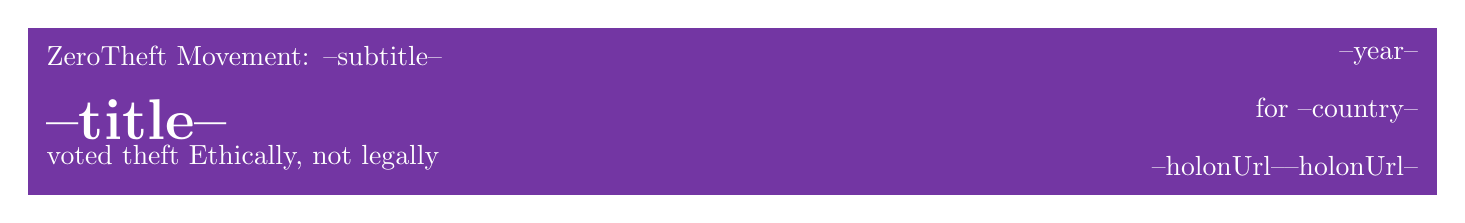
\begin{tikzpicture}
      \node[leftHeaderText] (subtitle) {ZeroTheft Movement: --subtitle--};
      \node[leftHeaderText, below=of subtitle, below=5pt] (title) {\huge \textbf{--title--}};
      \node[leftHeaderText, below=of title, below=-5pt] (belowtitle) {voted theft Ethically, not legally};

      \node[rightHeaderText, right=of subtitle] (year) {--year--};
      \node[rightHeaderText, below=of year, below=5pt] (country) {for --country--};
      \node[rightHeaderText, below=of country, below=5pt] (holon) {\href{--holonUrl--}{\color{white}--holonUrl--}};
    
      \begin{scope}[on background layer]
      \node[fill=primary, fit=(subtitle)(title)(belowtitle)(year)(country)(holon)] (header) {};
      \end{scope}
  \end{tikzpicture}
}

\trimbox{-120pt -15pt 0 0}{ 
  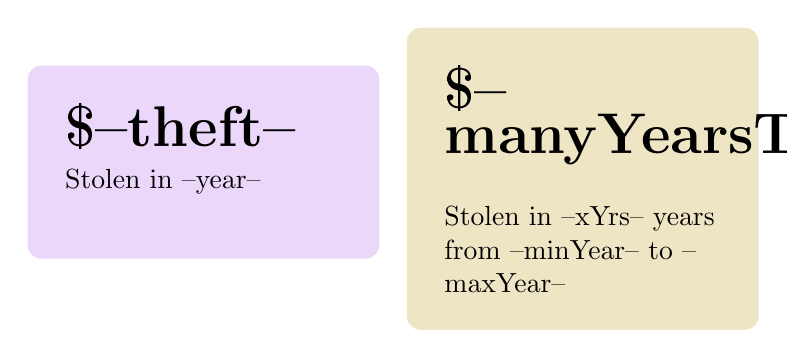
\begin{tikzpicture}
      \node[theftBlockContent] (amount1) {\huge \textbf{\$--theft--}};
      \node[theftBlockContent, below=0ptof amount1] (year1) {Stolen in --year--\newline};
      
      \begin{scope}[on background layer]
      \node[theftBlock, fill=theftBgColor1, fit=(amount1)(year1)] (block1) {};
      \end{scope}

      \node[theftBlockContent, right=30ptof amount1] (amount2) {\huge \textbf{\$--manyYearsTheft--}};
      \node[theftBlockContent, below=0ptof amount2] (year2) {Stolen in --xYrs-- years\\from --minYear-- to --maxYear--};
      
      \begin{scope}[on background layer]
      \node[theftBlock, fill=theftBgColor2, fit=(amount2)(year2)] (block2) {};
      \end{scope}
  \end{tikzpicture}
}

\trimbox{25pt -40pt 0 0}{
  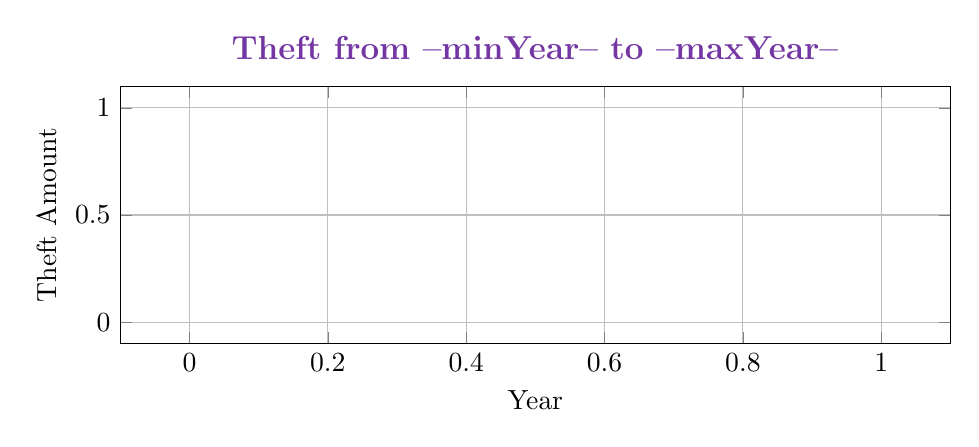
\begin{tikzpicture}
    \begin{axis}[
      title style={at={(0.5,1)},anchor=south,text=primary},
      title = \large \textbf{Theft from --minYear-- to --maxYear--},
      xlabel={Year},
      ylabel={Theft Amount},
      % xmin = 0, xmax = 10,
      % ymin = 0, ymax = 1,
      grid = both,
      % xtick distance = 1,
      x tick label style={/pgf/number format/.cd,%
        scaled y ticks = true,
        set thousands separator={},
        fixed},
      width = \textwidth,
      height = 0.4\textwidth,
      legend cell align = {left},
      % legend pos = north west,
      legend style={at={(0.5,-35pt)},anchor=north},
      scatter/classes={
      voting={theftValueType1Color, /tikz/mark size=3pt},%
      incompletevoting={theftValueType2Color, /tikz/mark size=3pt},%
      estimation={theftValueType3Color, /tikz/mark size=3pt}}
    ]
    
    \addplot[
      scatter,mark=*,primary,
      text=primary,
      scatter src=explicit symbolic,
      nodes near coords*=\scriptsize \textbf{\Theft},
      every node near coord/.append style={below right, rotate=90, shift={(0, 6pt)}},
      visualization depends on={value \thisrow{Theft} \as \Theft},
    ] 
    table [meta=DeterminedBy] {
      --theftValueChartData--
      % Year theft DeterminedBy Theft
      % 1    0.3  voting       0.25T   
      % 2    0.1  estimation       1.5    
      % 3    0.6  voting      0.70   
      % 4   0.4  incompletevoting      0.125  
      % 8   0.1  estimation       2      
    };
    
    \legend{
      % voting
      Voted Theft, 
      % incompletevoting
      Interim Theft (needs more vote),
      % estimation
      Estimated Theft
    }
    
    \end{axis}
  \end{tikzpicture}
}

\textcolor{primary}{\huge \textbf{Sources of theft}}
\setlength{\tabcolsep}{10pt} % for the horizontal padding
{\renewcommand{\arraystretch}{2}% for the vertical padding
    % \begin{longtable}{| p{150pt} | p{100pt} | p{100pt} | p{100pt} |} 
\begin{longtable}{p{150pt} p{100pt} p{100pt} p{100pt}} 
    % \hline
    \cellcolor{tableHeaderBg} \textbf{Problem Area} &
    \cellcolor{tableHeaderBg} \textbf{Vote} &
    \cellcolor{tableHeaderBg} \textbf{View More} &
    \cellcolor{tableHeaderBg} \textbf{Theft} \\ 

    --sourcesOfTheft--
    % \textbf{USA} & \cellcolor{tableTheftBg} \color{white} \centering \textbf{Theft 45\%} & \href{http://google.com}{Page 1} & needs 300 more votes \\
    % \quad \textbf{Economic Crisis} & \cellcolor{tableNoTheftBg} \color{white} \centering \textbf{Not Theft 45\%} & Page 10 & \$34B \\
    % \textbf{Bailouts} & \cellcolor{tableTheftBg} \color{white} \centering \textbf{Theft 45\%} & Page 1 & needs 300 more votes \\
    %\caption{Your caption here} % needs to go inside longtable environment
    % \label{tab:myfirstlongtable}
\end{longtable}
}
\end{document}
